% ================================================ %
% Headers and metadata
% ================================================ %

\documentclass[10pt,conference,compsocconf]{IEEEtran}

\usepackage{hyperref}
\usepackage{graphicx}	% For figure environment
\usepackage{amsmath}
\usepackage{algpseudocode}

\begin{document}
\title{%
    Discrete traffic data generation using ML methods \\
    \large \textit{CS-433 Machine learning -- Project 2}
}

\author{
  Luca Bataillard, Julian Blackwell, Changling Li\\
  \textit{School of Computer and Communication Sciences, EPFL}
}

\maketitle


% ================================================ %
% Abstract
% ================================================ %

\section*{Abstract}

This paper introduces a way to generate synthetic discrete traffic data for use in traffic
simulators. We present a model capable of taking historical traffic data from a given week and
predicting the discrete arrival times of vehicles in the same week, one year later. This is achieved 
using two phases. In the first phase, a recurrent neural network predicts the arrival rate for each 
hour in the week. In the second phase, a custom discretization model transforms our rates into new 
discrete arrival times. Our model outperforms our baseline in predicting arrival rates, and is 
...TODO in generating arrival times.


% ================================================ %
% Introduction
% ================================================ %

\section{Introduction}

Traffic simulators like SUMO \cite{SUMO2018} need vehicle data to perform modelling tasks. These
simulators are widely used in the fields of civil engineering and urban planning for modelling
complex traffic systems. They can provide city-wide traffic forecasts, allow for the evaluation 
of novel traffic control systems, or can even model the effect of autonomous vehicles on traffic
patterns. 

To simulate traffic flow, simulators will generate simulated vehicles on a given road based on a 
log of the speed and arrival time of vehicles on that road. Such real world data is obtained using 
a car sensor placed on or near the roadway. These sensors are not always online: they can break 
down or can be moved to be used elsewhere. They also cannot predict future traffic trends. This 
means that the logs sometimes have large gaps if using real-world data.

In this paper, we present a way to fill in the gaps in traffic logs and to predict future traffic 
logs up to a year in advance, using machine leaning models. Our model takes a week-long traffic
log and outputs a traffic log for the same week one year later. It can be combined to predict an 
entire year in parallel using data from the previous year. 

The model we propose has two phases, a rate prediction phase and a discrete event generation phase.
In the first phase, we predict a vehicle arrival rate for every hour in the week, using a LSTM 
recurrent neural network \cite{LSTM}. The second phase takes the hourly rates and outputs a discrete 
arrival log. It first predicts a 5-minute interval arrival rate using historical averages, then samples
a Poisson distribution to generate discrete events.

TODO + challenges + results

% ================================================ %
% Exploratory data analysis
% ================================================ %

\section{Exploratory data analysis}

We first start with some exploratory data analysis to better understand our time series data before further processing. Our dataset contains quite a few features but we mainly focus on the road caracteristics (lane, direction), the weight, speed, number of axles, type and crossing times of each vehicule. 

\subsection{Initial exploratory data analysis}

Our data ranges from 2011-04-01 00:41:31 to 2021-03-28, ranging a period of about ten years. We first find that all vehicles (or events) drive in the same direction. We then decide to discard this column. The minimum measured weight is 3.5t, which means that the vehicles are mainly heavy trucks. There are 2 lines, one that has less traffic than the other. We suppose that this is due to the fact that vehicles drive on the right lane and overtake on the left lane.

We then find that the number of axles is quite correlated to the weight, we decide to stop focusing on this feature. From several plots of weight and speed throughout a year, a month, a week and some days, we notice some repetitive trends. There is less traffic during the week-ends and the nights and the speed drops significantly around 5pm during the workdays. We suppose this is because of traffic jams. We also notice that the speed is quite constant from 6am to 5pm. 

Finally, there are 272 types of vehicles. They are classified by the number and location of axles on the car (type 121 means that it has one axle on the front, 2 axles in the middle and 1 axle on the back). We notice the weight is not quite the same for every type of vehicle which is not helpful to. We then decide to discard this feature for now to only focus on the speed, weight and crossing times of the vehicles.

A REVOIR/COMPLETER AVEC LA PARTIE DATA EXPLORATION DU NOTEBOOK 5

\subsection{Missing data points and further analysis on weight and speed}

We notice some periods of time with missing data points, specially towards the start of the COVID pandemic so we decide to omit this time period. After some inspections of the monthly number of vehicles per year (see Fig. 1 below), there are entire months with no data particularly in 2013 and 2014. \par

\begin{figure}[ht]
  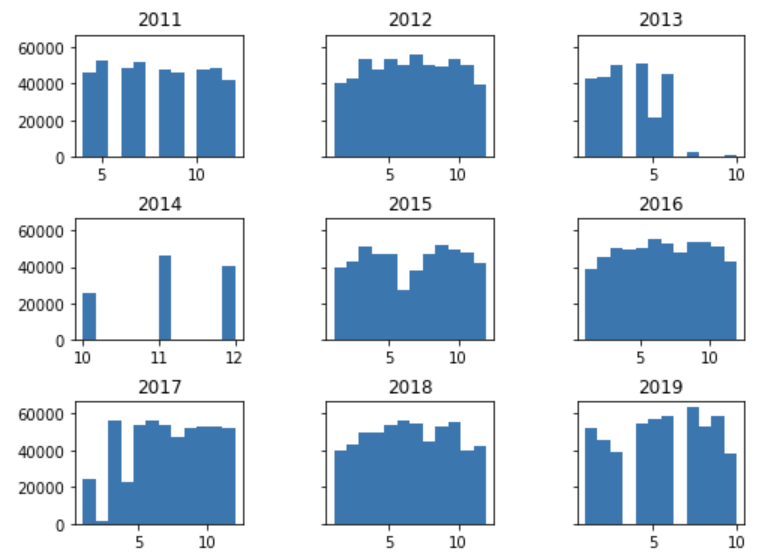
\includegraphics[scale = 0.63]{report/img/monthly-number-vehicles-per-year.png}
  \caption{Monthly number of vehicles per year. Horizontal axis corresponds to the month, the vertical axis to the number of vehicles per month.}
  \label{monthly-number-of-vehicles-per-year}
\end{figure}

We then investigate on possible relationships between speed, weight and time. We observe that a large majority of vehicles are bunched together between 65 and 100 km/h. After a quick look on the weight distribution among the vehicles, the weight is heavily left-tailed, with some rare exceptions weighing > 50 tons. We also find that the mean weight approximately varies between 16'000kg around 17'000kg for each month. 

After some analysis on a possible correlation between weight and speed, it does not seem like there is quite a significant correlation between speed and weight of a vehicle, there are slight differences in the distribution for certain weight ranges, so we should keep this in mind while generating a probability distribution for speed given a weight range.

\subsection{Year-on-year traffic increases}

Since the goal of our model is to make predictions up to a year in advance, we would like to first observe whether there already is a year-to-year trend. In order to do so, we fit a linear regression to investigate whether trend for the number of vehicles over time exists. 

We first observe significant variance in the data. The number of vehicles has a standard deviation $\sigma \approx 270$, and data points are on average very far from the fitted trend (with $R^2 = 0.029$). Keeping this in mind, simply training a model that minimises loss is unlikely to generate predictions with such variance (as outputting the mean achieves the lowest average error). To combat this, we will incorporate a probabilistic component to our model to better replicate fluctuations. 

Finally, the regression fit suggests an upwards trend in traffic over time with the number of vehicles climbing from approximately $10'000$ to $\sim 12'000$ per week. The gradient estimates an average increase of $3.353$ vehicles per week over the course of our data. 

% ================================================ %
% Feature engineering
% ================================================ %

\section{Feature engineering}

The raw data given to us is structured as a time series of discrete events. Each row represents 
a vehicle arrival and contains a timestamp of the arrival, the vehicle speed, and the vehicle 
weight. Other measurements such as lane of travel are discarded as they are not relevant for 
our main prediction task. We will reshape and expand these inputs and add new meaningful 
features to feed into our model. 

\subsection{Re-sampling}

The first step in our model is to predict a rate of vehicles, so we transform our data from discrete
events into an hourly arrival rate. We split the discrete data into intervals of 1h, so that our dataset
is indexed by a fixed timestep of 1h over the whole range of time. We call this interval our \textit{sampling interval}. 

We count the number of vehicles in each sampling interval to create the \texttt{n\_vehicles} column. The speed and weight of the discrete events in the interval are also aggregated by a sum to create the total \texttt{speed} and \texttt{weight} columns.

As a precaution, we filter out the dates past October 21st 2019 to avoid the unpredictable changes in traffic patterns due to the COVID-19 pandemic. We chose this exact date because it is the last non-zero
data point until January 1st 2020, after which we consider the pandemic to have started.

\subsection{HGV Driving restrictions}

Heavy goods vehicles (\textit{HGV}) in Switzerland are forbidden to drive on Sundays and on weekdays from 10 PM to 5
AM. Since our data only includes vehicles over 3.5 tonnes, we need to take this into account. We add a
binary \texttt{is\_legal} feature whose value is 1 if it is legal for a HGV to drive and 0 otherwise.

\subsection{Time periodicity}
At the moment, the event timestamps are not very useful in their string representation. We would like to let our model consider any patterns in time, notably at the same hour of day (e.g. 7AM vs. 4PM), day of the week (e.g. Monday vs. Saturday), and time of the year (e.g. Christmas vs. summertime). Being traffic data, the rate of vehicles is clearly affected by these. In order to do so, we convert the timestamp into seconds, and apply a sine and cosine transform to obtain a periodic signal with respect to a wanted interval:
\[ 
\textrm{\textit{transform}(timestamp)} = \begin{cases}
    \sin \left( \textrm{timestamp} \times \frac{2\pi}{L} \right) \\
    \cos \left( \textrm{timestamp} \times \frac{2\pi}{L} \right)
\end{cases}
\]
where the \textbf{timestamp} input has already been converted into seconds and $L$ is the interval length in seconds (e.g. for a day, $L=60*60*24=86400$ seconds). One can uniquely reconstruct the date and time within a year from the transformed signals. 

\subsection{Splitting and normalising}

We split our data into a training, validation and test dataset. The test and validation datasets contains two years of data each, the training set gets the remaining 4.4 years. Each year is considered to be 52 weeks long exactly in order to simplify windowing. 

We standardise our features in each of the datasets by subtracting each feature from its mean and dividing it by its standard deviation in the training set. 

\subsection{Windowing}

In order to create more data samples into our model, we use the concept of a sliding time window.
We create a window object to generate our model inputs and outputs. This object takes a dataset and 
splits it into (input, output) tuples. Is does so as follows:
\begin{enumerate}
    \item  It specifies a window of (1 year + 1 week). The input data will be the first week of the
    window, the output the last. This means that our model will predict a week using the same week 
    of the previous year.
    \item  It takes the dataset and slides the window along the dataset, one hour at a time. 
    Each slide creates a new (input week, output week) tuple.
    \item It creates a new dataset from the generated tuples. The tuples are shuffled and batched into
    batches of 32. We feed the network one entire batch at a time. This is equivalent to performing
    stochastic gradient descent with minibatches, which reduces training time.
\end{enumerate}

\subsection{Zero weeks filtering}

As seen in the exploratory data analysis section

It filters (input, output) tuples if either the input or the output number of vehicles is 0 for the whole week. It does so when transforming the data from from a Pandas DataFrame to a TensorFlow Dataset.

% ================================================ %
% Model structure and selection
% ================================================ %

\section{Model structure and selection}

\subsection{Rate prediction}

Our task is to use the hour-by-hour features described above from the input week to predict the
vehicle count, sum of speeds, and sum of weights for our output week. We evaluated several
possible models against our baseline to find the best performing model. We used mostly default 
configurations for our models. 

Our baseline consists of outputting the same values from the previous week. We compare 
our models to it by computing the Mean Squared Error and Mean Absolute Error between the 
predicted week and the target week. 

Our models are built using the Keras \cite{keras} API for Tensorflow \cite{tensorflow}. They 
all use the default gradient descent algorithm provided by Keras and use early stopping evaluated 
on the validation dataset to avoid overfitting.

The models take a $H \times F$ matrix as input and output a $H \times N$ matrix. Here, $H = 168$ 
is the number of hours in a week, $F = 10$ is the number of input features, and $N = 3$ is the
number of output features (\texttt{n\_vehicles}, \texttt{speed}, \texttt{weight}).

We evaluated the following models:

\subsubsection{Linear model}

A linear regression model without regularisation 

\subsubsection{Neural Network}

A neural network with a single hidden layer of 512 neurons and ReLU activation.

\subsubsection{LSTM}

A recurrent neural network with a layer of 32 LSTM cells, followed by a fully connected layer.


\subsection{Discrete event generation}

Once we have predicted a rate of vehicles passing in each time interval, we now have to generate discrete events. We will work upon the assumption that vehicle arrival times are drawn from a real-world stochastic process. Our aim is to draw samples from the same distribution to get random but representative results.

We can simulate such events with a Poisson process \cite{poisson} with rate equal to the predicted vehicle rate. However, if one has a look at the given vehicle arrival data, the rate is not necessarily uniform over an hour-long time interval. Most notably, this is quite noticeable early in the morning and late in the evening, where one can respectively observe an "acceleration" and "deceleration" in vehicle arrival rates.

To improve the

Finally, once a rate has been assigned to each 5-minute interval, one can finally generate arrival times with the following Poisson process (adapted from Prof. M. Bierlaire \cite{poisson}):
\begin{algorithmic}[1]
    \State $A \gets $ empty list
    \State $t = 0$
    \State Draw $r \sim U(0,1)$
    \State $t = t - \ln(r) / \lambda$
    \State \textbf{if} $t > T$ \textbf{return} A
    \State A.append(t)
    \State \textbf{GOTO} step 3
\end{algorithmic}

where $U\sim(0,1)$ is the uniform distribution between 0 and 1, $\lambda$ is the rate, and $T$ is the 5-minute time length ($300$ seconds).


% ================================================ %
% Experimental results
% ================================================ %

\section{Experimental results}

In this section, we show the results of our  

\subsection{Rate prediction performance}

We evaluated the mean squared error and mean absolute error of our trained models on our test set. We 
also computed the relative difference with respect to our baseline for each metric.
We obtained the following results:

\begin{table}[h!]
\begin{center}
    \begin{tabular}[c]{| c| c c | c c | }
        \hline
         \textbf{Model} & \textbf{MSE} & \% & \textbf{MAE} & \%\\
         \hline
         Baseline    & $0.3430$ &   -       & $0.2959$ & -\\
         Linear      & $0.3753$ & $+\,9.43$ & $0.4186$ & $+41.47$ \\
         Neural Net. & $0.3273$ & $-\,4.57$ & $0.3596$ & $+21.54$ \\
         LSTM        & $0.2889$ & $-15.78$  & $0.3264$ & $+10.32$  \\
         \hline
    \end{tabular}
\end{center}
\label{table:ratepred}
\caption{MSE and MAE loss on test set for each model.\\
{\footnotesize \% is the relative difference to baseline}}
\end{table}

TODO Smooth baseline

\subsection{Sampling interval selection}

As discussed in the exploratory data analysis section, our data exhibits significant changes in arrival
rates between hours.  We therefore did not consider sampling intervals (the time step for which we count the number of vehicles) larger than 1h . It would make the second phase of our prediction model harder. However, we still 
wish to determine appropriate sampling intervals to predict vehicle arrival rates. 

We also have to consider the trade-off between computation time and model performance. We evaluated our
best performing model on a 1 hour, 30 min, and 10 min sampling interval. We also considered evaluating a
2 min interval, but its computation time was too great on our machines.

After evaluating our selected LSTM model on different sampling intervals, we obtained the following results:

\begin{table}[h!]
\begin{center}
\begin{tabular}{| c| c c c | }
\hline
 \textbf{Interval}   & 1h & 30 min & 10 min \\
 \hline
 \textbf{MSE (Val)} & $0.261$ & $0.268$ & $0.317$ \\
 \hline
\end{tabular}
\end{center}
\label{table:sampling}
\caption{MSE of LSTM for different sampling rates.\\
{\footnotesize \% is the relative difference to baseline}}
\end{table}

We see that predictive performance decreases with smaller sampling intervals. We therefore choose to sample our
weekly discrete data over a period of 1h. This strikes a good balance between the predictive power of our rate
prediction model and the performance of our discrete generation phase, while also taking computation time into account. 

\subsection{Discrete event generation performance}

% ================================================ %
% Future work
% ================================================ %

\section{Future work}

\subsection{Not treating weeks as independent}

\subsection{Improved Poisson process}

\subsection{TODO...}


% ================================================ %
% Conclusion
% ================================================ %

\section{Conclusion}


% ================================================ %
% Bibliography
% ================================================ %


\bibliographystyle{IEEEtran}
\bibliography{report}

\end{document}